%
%% This is file `sample-sigconf.tex',
%% generated with the docstrip utility.
%%
%% The original source files were:
%%
%% samples.dtx  (with options: `sigconf')
%% 
%% IMPORTANT NOTICE:
%% 
%% For the copyright see the source file.
%% 
%% Any modified versions of this file must be renamed
%% with new filenames distinct from sample-sigconf.tex.
%% 
%% For distribution of the original source see the terms
%% for copying and modification in the file samples.dtx.
%% 
%% This generated file may be distributed as long as the
%% original source files, as listed above, are part of the
%% same distribution. (The sources need not necessarily be
%% in the same archive or directory.)
%%
%% Commands for TeXCount
%TC:macro \cite [option:text,text]
%TC:macro \citep [option:text,text]
%TC:macro \citet [option:text,text]
%TC:envir table 0 1
%TC:envir table* 0 1
%TC:envir tabular [ignore] word
%TC:envir displaymath 0 word
%TC:envir math 0 word
%TC:envir comment 0 0
%%
%%
%% The first command in your LaTeX source must be the \documentclass command.
\documentclass[sigconf,nonacm]{acmart}

\newcommand{\scores}{\textsc{SCORES}}

\usepackage{verbatim}
\usepackage[linesnumbered, boxed, resetcount]{algorithm2e}
\usepackage{appendix}
\usepackage{hyperref}
\usepackage{cleveref}
\usepackage{dblfloatfix}

%%
%% If you need any other LaTeX packages, add them here
%%

%%
%% end of the preamble, start of the body of the document source.
\begin{document}

%%
%% The "title" command has an optional parameter,
%% allowing the author to define a "short title" to be used in page headers.
\title{Human-perceived Difficulty of Chess Positions: Survey and Preliminary Experiments}


%%
%% The "author" command and its associated commands are used to define
%% the authors and their affiliations.
%% Of note is the shared affiliation of the first two authors, and the
%% "authornote" and "authornotemark" commands
%% used to denote shared contribution to the research.
\author{Zala Urh}
%\authornote{All three authors contributed equally to this research.}
\email{zu0476@student.uni-lj.si}
\affiliation{%
    \institution{Faculty of Computer and \\Information Science,\\
    University of Ljubljana\\Ve\v{c}na pot 113}
    \city{SI-1000 Ljubljana}
    \country{Slovenia}
}

\author{Matej Belšak}
%\authornotemark[1]
\email{mb4390@student.uni-lj.si}
\affiliation{%
    \institution{Faculty of Computer and \\Information Science,\\
    University of Ljubljana\\Ve\v{c}na pot 113}
    \city{SI-1000 Ljubljana}
    \country{Slovenia}
}

\author{Luka Bajić}
\email{luka.bajic@fri.uni-lj.si}
\affiliation{%
    \institution{Faculty of Computer and \\Information Science,\\
    University of Ljubljana\\Ve\v{c}na pot 113}
    \city{SI-1000 Ljubljana}
    \country{Slovenia}
}

\author{Ivan Bratko}
\email{ivan.bratko@fri.uni-lj.si}
\affiliation{%
    \institution{Faculty of Computer and \\Information Science,\\
    University of Ljubljana\\Ve\v{c}na pot 113}
    \city{SI-1000 Ljubljana}
    \country{Slovenia}
}

%%
%% The abstract is a short summary of the work to be presented in the
%% article.
\begin{abstract}
In this paper we survey existing approaches for estimating difficulty of chess positions as perceived by human players. Additionally, we offer our own implementation of rating prediction on chess puzzles using hand-crafted features, primarily based on the properties of the search tree and on performance of weak engines. We explain both classifiers and regressors using SHAP. 
\end{abstract}

%%
%% Keywords. The author(s) should pick words that accurately describe
%% the work being presented. Separate the keywords with commas.
\keywords{chess, explainability, classification, regression, ranking, feature engineering}

%%
%% This command processes the author and affiliation and title
%% information and builds the first part of the formatted document.
\maketitle

\section{Introduction}

Explaining why a given chess position is perceived as easy or hard has been a long-standing goal both for human players and artificial intelligence researchers. This can be seen as a subset of the problem of explaining game states in general zero-sum two-player games. Possible applications of a solution to this problem range from tutoring software to automatic skill estimation in said games.

In this paper we overview existing approaches in this domain, as well as offer our own implementation of puzzle difficulty prediction. This problem could be formulated in many different ways, and could easily be seen as an interdisciplinary endeavor, however in this work we take a primarily machine learning view. In particular, we think of difficulty estimation as either a regression problem, where given an arbitrary chess position, we simply wish to predict its rating, or a a classification problem, where we should first bin all available positions into classes, say \textit{easy}, \textit{medium}, and \textit{hard}. 

A possible issue with such approaches is the apparent subjectivity of rating assignment, however it will become clear that the process is not unlike assigning ratings to human players and adjusting them based on tournament, or individual game performances, which seems to be a generally accepted method of estimating players' skill level. 

Another possible approach would be to avoid numerical ratings altogether, and instead treat difficulty estimation as purely a ranking problem. In this paradigm, the model should simply state which of the given two (or more) positions is perceived as more difficult. However, it is clear that this does not eliminate subjectivity whatsoever. 

\section{Related work}

In recent years we have observed an increased interest in the problem of predicting puzzle difficulty, largely due to the IEEE BigData 2024 Cup \cite{competition2024} and the FedCSIS 2025 knowledgepit.ai Competition \cite{competition2025}, both of which focused precisely on this topic. 

The best performing models in both cases belonged either to the deep learning paradigm, e.g. \cite{compdl, compdl2}, or to the gradient boosting family, e.g. \cite{compgb}. Interestingly, even the former approaches often utilized hand-crafted features, which is seldom seen in other fields, however it is a good indication of the difficulty of this problem.  

A number of hand-crafted features are also described in \cite{bratko2, bratko, bratko3}. Here the idea is to use the breadth and depth of the search tree explored by the engine as a proxy for the difficulty of the given position. For this approach to work, the pruning should coincide with the human thinking process, e.g. checks, and captures should be considered no matter what, while certain nonsensical moves can be rejected instantly without further search. 

\subsection{Human-play Modelling}

Since chess engines started surpassing the skill of human players by a large margin, attention has somewhat shifted to developing engines that exhibit a more human playing style with the purpose of making the moves more intuitively understantable. This is by no means a solved problem, as it is difficult to even quantify what constitutes a human-like playing style. 

Arguably the first big breakthrough in this regard was the AlphaZero engine \cite{alphazero}, which was trained purely via self-play, and was claimed to produce more human-like moves compared to other state-of-the-art engines at the time. This claim, as well as the possible drawbacks, were discussed, for instance, in \cite{bratkoalpha}. 

Other noteworthy human-modelling engines come from the Maia family, namely Maia-1 \cite{maia1}, Maia-2 \cite{maia2}, and Maia-3 \cite{maia3}. The latter, in particular, simultaneously models human play, maximizes playing strength and offers interpretability. 

ALLIE \cite{allie} is yet another recent attempt at modelling human play, with particular emphasis on modelling a sequence of moves before the current move. Similar approach can be seen in Otter \cite{otter}, but with additional capability of modelling clock management. 

\subsection{Machine Learning for Tabular Data}
\label{ml_tab}

Recently, substantial progress has been made in the field of machine learning for tabular data, which can be seen for instance on the TabArena benchmark \cite{tabarena}. Recent foundational models such as Kumo-Tabular \cite{kumo} and TabFM \cite{tabfm} have surpassed previous state-of-the-art models such as XGBoost \cite{xgboost}, CatBoost \cite{catboost}, LightGBM \cite{lightgbm}, and their variants, all based on the gradient boosting paradigm. Importantly, these models work out-of-the-box, i.e. require no additional domain-specific fine-tuning.

\subsection{Engine Strength Estimation}

The problem of assigning a rating to chess engines has been of interest even before their level of play was comparable to that of a human \cite{comprating1, comprating2}. The initial belief was that an estimated Elo rating grows linearly with the depth of engine's search capabilities, i. e. that adding a ply of depth increases the engine's Elo by a constant. Due to hardware limitations, diminishing returns of increasing search depth were only observed later, e.g. in \cite{comprating3}. 

Currently, engines are evaluated according to the Elo rating system, with rating changing based on tournament play, e.g. \cite{engine, engine2, engine3}. However, engine tournaments are not universally standardized, and can use different time controls, hardware, etc. which means that ratings from one engine to another are not necessarily comparable. They are certainly not directly comparable with human ratings either, despite using the same rating system. 

\subsection{Explainability}

Chess has proven to be a relevant and relatively challenging domain for Explainable AI (XAI). A lengthy survey of recent approaches can be found in \cite{xaichesssurvey}, for a more general XAI survey, see \cite{xaisurvey}. 

State-of-the-art machine learning models, including those discussed in Section~\ref{ml_tab}, typically do not offer any inherent explanation for their decision. This is true both for classifiers and regressors, and is especially problematic in the deep learning paradigm, where even the features are usually computed by the model itself, i.e. without human input. The lack of human-understandable features makes it difficult to infer the reasoning behind the output produced by the model. Nonetheless, several approaches to alleviate this problem have been developed. 

SHAP \cite{shap} is a model-agnostic explainer, meaning the explanation is not tied to the specifics of a given classifier or regressor. This is beneficial because we can thus use the same method to evaluate vastly different models. A high level overview of SHAP is the following: to determine the importance of each individual feature, we can iteratively corrupt different subsets of features (e.g. by setting them to the corresponding mean values) and observe the change in the output of the model. If the change is substantial, the corrupted features were important. Since there are exponentially many subsets of features, Monte Carlo techniques are often used for efficiency. Details of this approximation are discussed in \cite{shapopt}. 

\section{Methodology}

\subsection{Data}

To train and evaluate our models, we use a subset of the Lichess puzzle dataset \footnote{https://database.lichess.org/\#puzzles} containing 3000 puzzles with ratings ranging between 399 and 3092. We discard all columns except FEN, rating, and themes. Furthermore, we only keep a subset of themes which have a precise definition (for a full list, see the implementation \footnote{Full implementation is available at https://github.com/bajicluka01/chess-puzzle-evaluation/tree/main}). For classification we create classes "easy", "medium" and "hard" by splitting this interval equidistantly. The dataset is split into training set and test set with the ratio 80:20. The data is standardized, meaning we transform it in such a way that it follows a standard normal distribution with zero mean and unit variance. This is required by distance-based models to ensure that each attribute is treated as equally important. 

The distribution with indicated bins for easy, medium, and hard classes, is shown in Figure~\ref{dist}

\begin{figure}
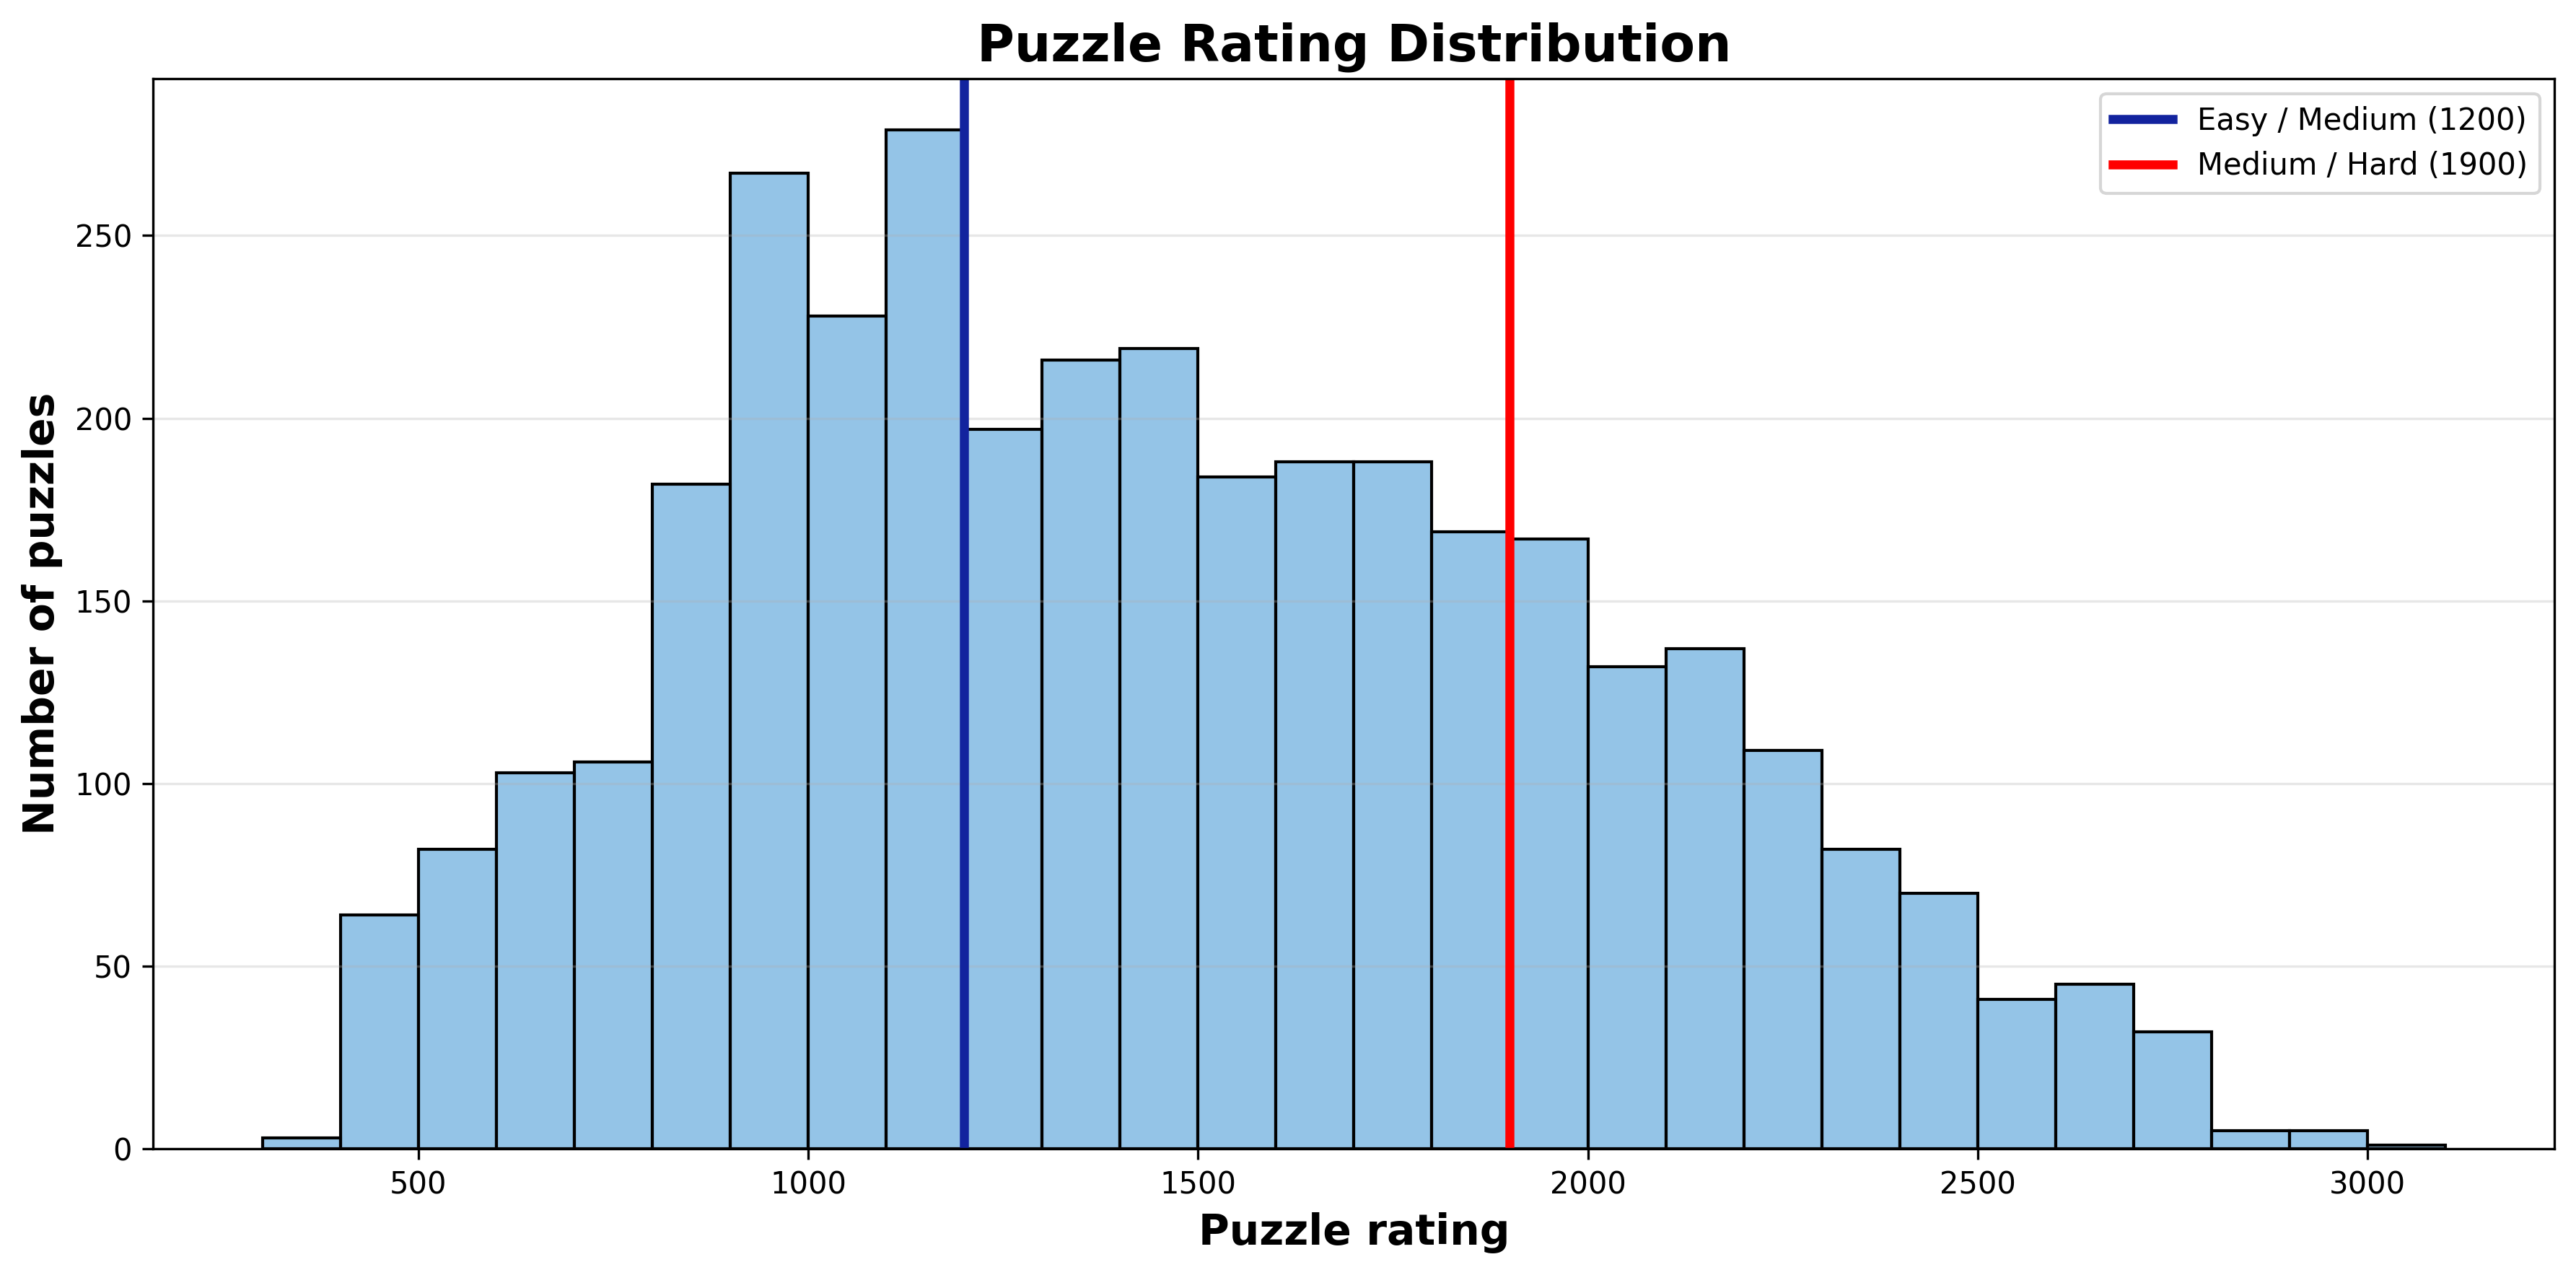
\includegraphics[width=1.0\linewidth]{plots/rating_distribution.png}
\caption{Rating distribution.}
\label{dist}
\end{figure}

\subsection{Evaluation Metrics}

For classification problem we use the standard metrics: classification accuracy, F1 score and AUC. For regression we use mean absolute error (MAE) because unlike mean squared error, it has a more intuitive interpretation on this dataset. We also report which percentage of the rating interval this MAE covers. For ranking we use Normalized Discounted Cumulative Gain (NDCG) and Kendall $\tau$ to determine the accuracy of the model's ranking against the ground truth, which is simply a ranking assigned by ordering the ratings in the dataset. 

\subsection{Features}

In this section we discuss the features that were used for model training in Chapter~\ref{results}.

\subsubsection{Meaningful Search Tree}

We use the features from \cite{bratko3} (except \textit{SeeminglyGood}, which is not rigorously defined and cannot be easily reproduced) with the following modification: we generate the \textit{MeaningfulMoves}  feature using Otter \cite{otter}, a recently developed engine that models human play, and use these moves to compute the remaining features from \cite{bratko3}. 

This change is motivated by the following: meaningful moves in \cite{bratko3} are intended to represent the moves a human player would generally consider in a given position (including moves that are quickly rejected, e.g. captures that obviously do not work). However, these moves are computed directly from the engine evaluation, which renders the feature useless in many cases, e.g. in tactical positions in which there is objectively only one good move, whereas a human player clearly needs to consider multiple alternatives. Conversely, Otter \cite{otter} is a transformer-based approach that for a given position $P$ returns a probability distribution across all legal moves in $P$, indicating how likely a human player is to consider each alternative. In other words, we obtain probabilities $p_i$ with the following properties:

\begin{equation}
\label{prob}
\forall i=1,\dots,k:\quad p_i\geq0, \quad\sum_{L(P)}p_i=1
\end{equation}

\noindent
where $L(P)$ is the set of legal moves in position $P$ and $i$ enumerates all the moves in $L(P)$, so $|L(P)|=k$. 

In our experiments we select meaningful moves by using an arbitrarily chosen cutoff $p_i>0.1$, which based on Equation~\eqref{prob} gives at most 10 (but typically less) moves most likely to be considered by a human player in a given position. In our view this coincides with the number of moves an expert player typically considers. 

\subsubsection{Weak Engines}

The following reasoning should make intuitive sense: if a weak engine (or player) can solve a given puzzle, it is more likely to be a low-rated puzzle. Therefore we can employ several weak engines and use indicators of their puzzle-solving success as a subset of features. What exactly is meant by "weak" is not of great importance (see discussion in Chapter \ref{elo_ch}) - in fact it is desirable to use multiple engines with varying estimated strengths \footnote{Note that using, e.g. Stockfish with different playing strength parameters, gives unsatisfactory results. Evidently, making a strong engine play at less-than-full strength, is a harder (and perhaps less interesting) problem than implementing a weak engine from scratch.} to obtain less correlated features. 

\subsubsection{Miscellaneous}

In addition to the above mentioned features, we also use Stockfish's outputs, namely centipawn evaluations, win/draw/loss rate and selective depth. 

Furthermore, we compute the number of pins and forks in the given position based on the following definitions.



\section{Results}
\label{results}

\subsection{Correlation between puzzle rating and engine Elo}
\label{elo_ch}

The quality of the Elo \cite{elo, eloo} rating system in chess has been called into question numerous times, e.g. in \cite{elo1, elo2}, however it remains a generally accepted measure of playing strength. In many settings, including Lichess (hence also in the dataset used in this paper), the Glicko-2 \cite{glicko_orig, glicko_example} rating system is used instead \footnote{Whether applying any rating system to an individual position rather than a player/engine even makes sense is a separate discussion, which we do not engage in here.}. On the other hand, estimation of chess engines' playing strength is generally still done using Elo \footnote{Furthermore, authors often estimate their engine's rating in non-standardized ways, which makes ratings across different engines difficult to compare}. Therefore it is worth investigating the correlation between an engine's rating and its ability to solve puzzles of a similar rating. 

The results are shown in Figure~\ref{corr}.

\begin{figure}
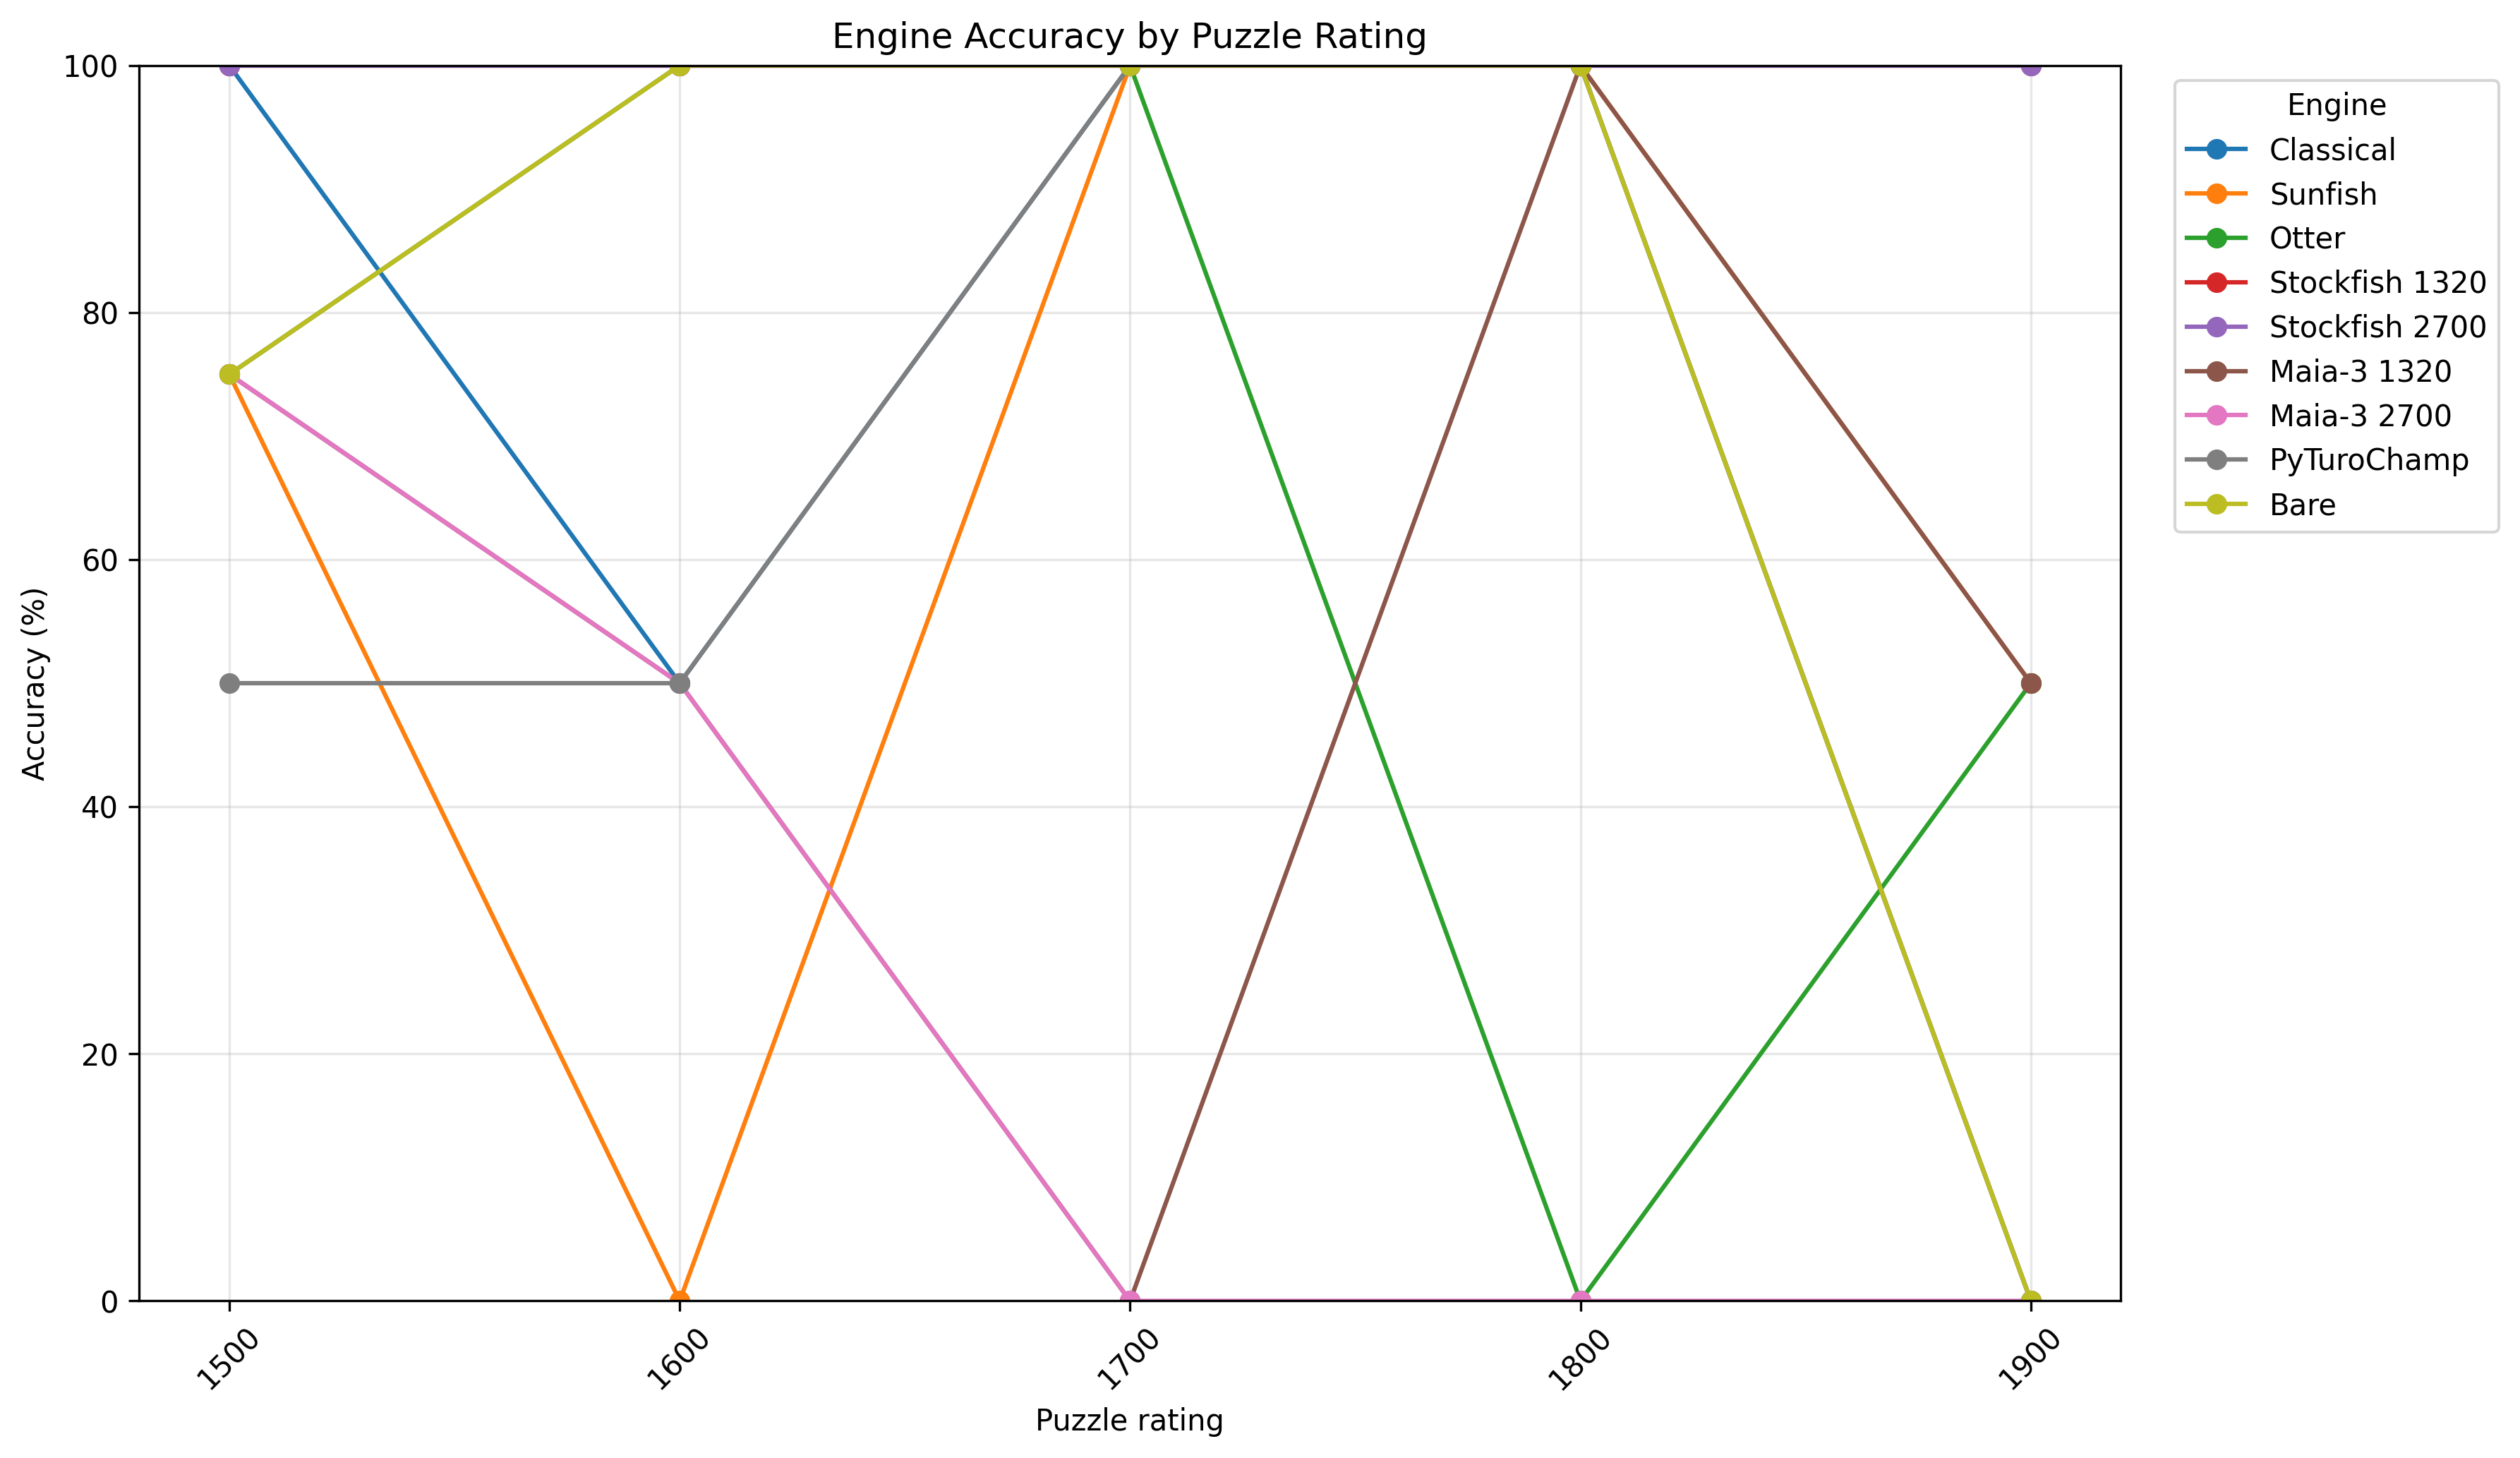
\includegraphics[width=1.0\linewidth]{plots/engine_plot.png}
\caption{Engine puzzle solving success based on puzzle rating.}
\label{corr}
\end{figure}

\subsection{Classification}

Table \ref{classification} displays the performance of the standard machine learning models \cite{scikit} on a dataset with 1000 samples and all available attributes. Class distribution is 39.1\% "easy", 38.9\% "medium" and 22.0\% "hard". 

XGBoost uses 100 estimators and learning rate 0.1. SVM uses regularization parameter $C=1$ and balanced class weight. Random Forest uses 100 estimators. kNN uses 10 nearest neighbors and Euclidean distance. MLP uses $layers=[2048, 1024, 512, 256, 128]$, ReLU activation function, ADAM solver, regularization $\alpha=0.001$ and batch size 512. Default values are used for all remaining parameters. Ensemble uses a soft voting scheme on the outputs of all other models, meaning that probabilistic predictions are aggregated and finally converted into a class value. Misclassifications are discussed in Appendix 2. 

\begin{center}
\begin{table}[!ht]
\caption{Classification scores on 1k dataset.
\label{classification}}
\centering
{\begin{tabular}{c|c|c|c}
model & CA & F1 & AUC \\ \hline
XGBoost & 0.575 & 0.574 & 0.756 \\
kNN & \textbf{0.635} & \textbf{0.621} & 0.773 \\
Random Forest & 0.620 & 0.616 & 0.772  \\
Gradient Boosting & 0.575 & 0.563 & 0.758  \\
MLP & 0.630 & \textbf{0.621} & 0.770 \\
SGD & 0.550 & 0.551 & 0.693 \\
SVM & 0.595 & 0.574 & 0.756 \\
Ensemble & 0.615 & 0.612 & \textbf{0.779} \\
\end{tabular}}
\end{table}
\end{center}

In Table \ref{class} we show the results of an ablation study aimed to determine the utility of each subset of attributes. We use the best performing model in terms of CA from the previous experiment: kNN with $k=10$. Baseline refers to simple attributes, such as centipawn evaluations and number of searched nodes for each depth. These attributes are used in each experiment. Study refers to attributes from \cite{bratko3}.

\begin{center}
\begin{table}[!ht]
\caption{Ablation study on 1k dataset.
\label{class}}
\centering
{\begin{tabular}{c|c|c|c}
model & CA & F1 & AUC \\ \hline
baseline & 0.565 & 0.561 & 0.671 \\
counts & 0.555 & 0.545 & 0.688 \\
study & 0.565 & 0.548 & 0.716 \\
Stockfish & 0.565 & 0.557 & 0.752 \\
themes & 0.565 & 0.554 & 0.704  \\
counts, study & 0.530 & 0.508 & 0.723 \\
counts, Stockfish & 0.575 & 0.563 & 0.716 \\
counts, themes & 0.565 & 0.553 & 0.713 \\
study, Stockfish & 0.580 & 0.561 & 0.766 \\
study, themes & 0.58 & 0.570 & 0.717 \\
all attributes & 0.635 & 0.621 & 0.773 \\
\end{tabular}}
\end{table}
\end{center}

This confirms the usefulness of attributes from \cite{bratko3} and also confirms the usefulness of themes. The contribution of solving success is negligible, possibly due to an inherent flaw in the implementation of Stockfish playing strength: weaker play is simulated by limiting the depth of the search tree and imposing a time constraint on the search, however, this might not accurately simulate the puzzle-solving ability of a player with a certain ELO, rendering the attributes useless. 

\subsection{Regression}

Regression results are shown in Table \ref{regression}. XGBoost uses 100 estimators and learning rate 0.1. MLP uses $layers=[256, 256, 128, 128, 128, 64]$, ReLU activation function,  adaptive learning rate, ADAM solver, regularization parameter $\alpha=0.001$ and batch size 256. Default values are used for all remaining parameters. Ensemble model performs unweighted averaging on the outputs of all other models. 

\begin{center}
\begin{table}[!ht]
\caption{Regression scores on 1k dataset.
\label{regression}}
\centering
{\begin{tabular}{c|c|c}
model & MAE & \% of interval  \\ \hline
XGBoost & 329.836 & 12.2 \\
Linear regression & 321.600 & 11.9  \\
MLP & 317.419 & 11.8 \\
Bayes Ridge & 314.587 & 11.7 \\
Ensemble & \textbf{310.385} & \textbf{11.5} \\
\end{tabular}}
\end{table}
\end{center}

\subsection{SHAP explanations}


\begin{figure}
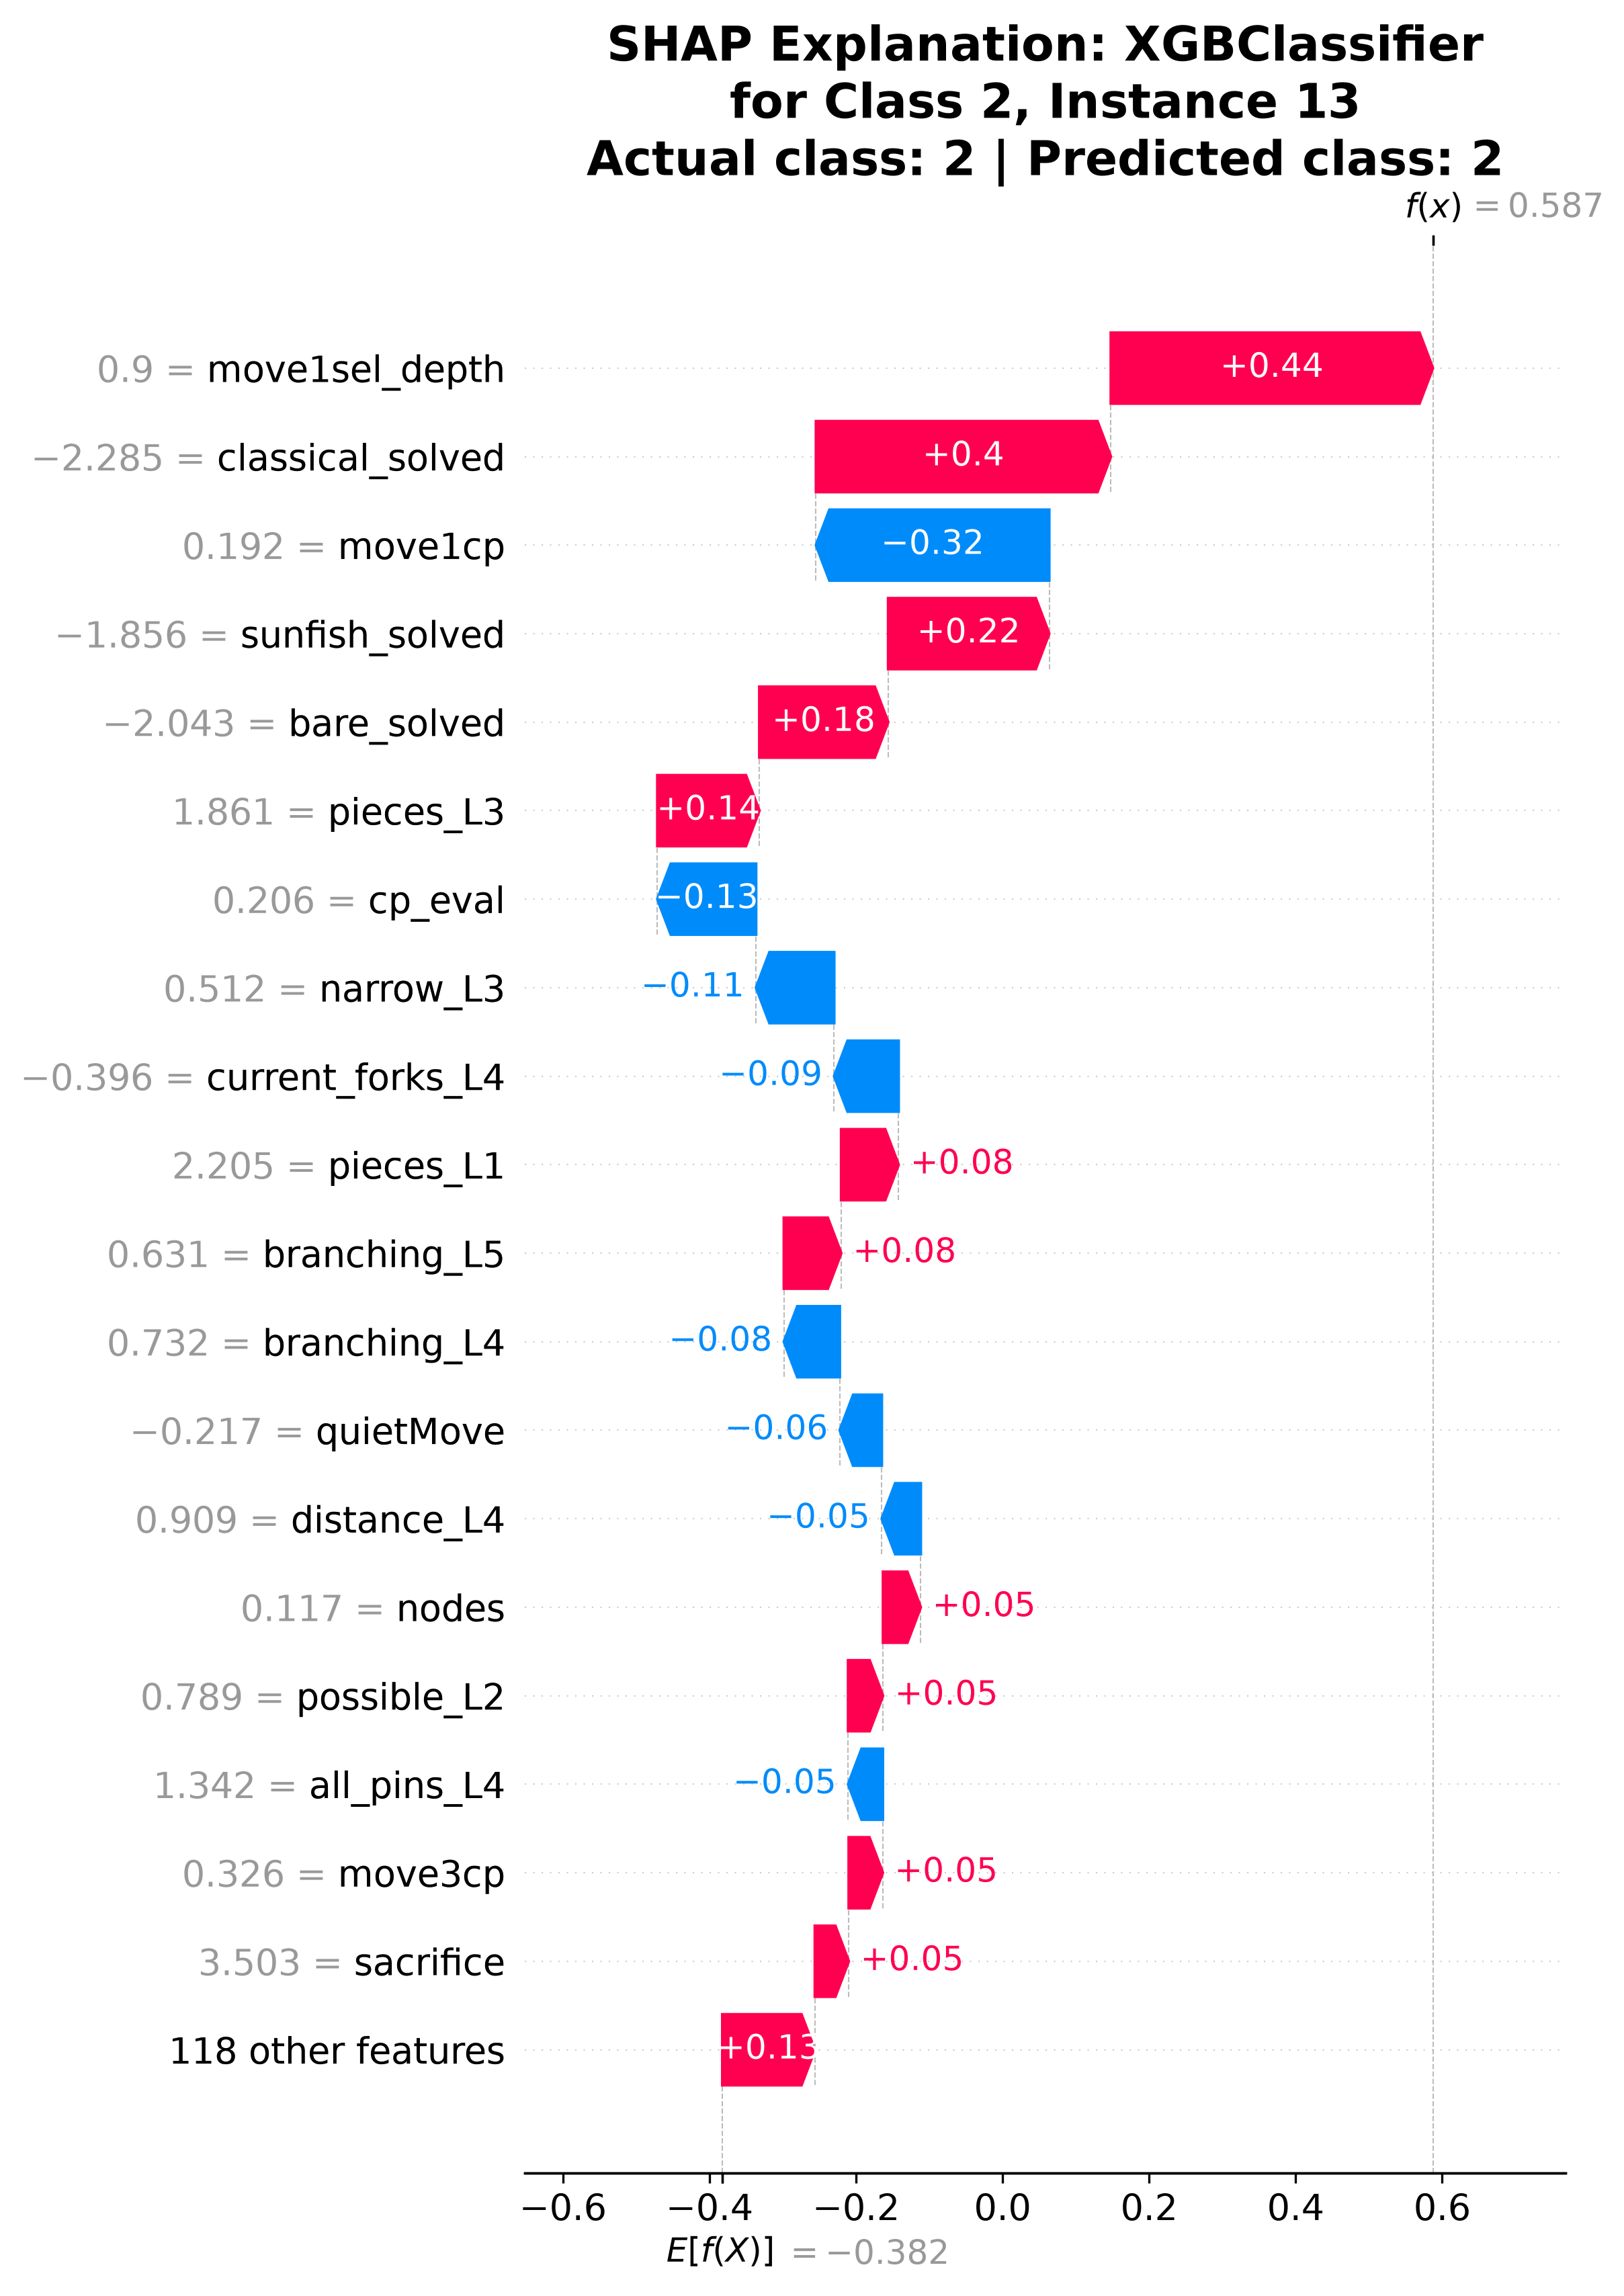
\includegraphics[width=1.0\linewidth]{plots/xgb_classifier_explanation.png}
\caption{XGBoost explanation}
\label{shap}
\end{figure}

\section{Discussion}

\subsection{Misclasifications}

\section{Conclusions}

Future work would consist of checking if these approaches are suitable also for strategic/nondescript positions, rather than just puzzles. Here, the main challenge is in assigning the ground truth ELO to these positions, since consensus among human players is more difficult to achieve. 

Additionally, Maia chess engine \cite{maia1} \cite{maia2} could be used as an alternative to Stockfish, as it is designed to approximate human play more closely. However, we ran a few experiments on known positions, and again this similarity to human-like play does not directly translate to human-like puzzle solving, so additional model training may be required, which is outside the scope of this paper. 

\bibliographystyle{ACM-Reference-Format}
\bibliography{references}

\appendix
%\begin{appendices}

%\section*{Appendix 1: attributes}
%\label{app1}

%\section*{Appendix 2: misclassifications}

%\section*{Appendix 3: interpretability}



%\end{appendices}

\end{document}
